% !TEX program = pdflatex
\documentclass[11pt]{article}

% Encoding & fonts
\usepackage[T1]{fontenc}
\usepackage[utf8]{inputenc}
\usepackage{lmodern}

% Layout & links
\usepackage[margin=1in]{geometry}
\usepackage{microtype}
\usepackage{hyperref}
\usepackage{adjustbox} 
\usetikzlibrary{positioning} 

% Math
\usepackage{amsmath,amssymb,amsthm}
\usepackage{mathtools}
\usepackage{enumitem}
\usepackage{array}
\usepackage{booktabs}
\usepackage{seqsplit}
% Figures
\usepackage{tikz}
% Tolerance for overfull lines
\setlength{\emergencystretch}{3em}

% Lean hook helpers (paper-side)
\newcommand{\LeanHook}[1]{\texttt{\seqsplit{#1}}}
\newcommand{\LeanRepoURL}{https://github.com/jonwashburn/lean-to-measurement}
% Common macros
\newcommand{\ph}{\varphi}
\newcommand{\lamrec}{\lambda_{\mathrm{rec}}}
\newcommand{\tauzero}{\tau_{0}}
\newcommand{\ftau}{\dfrac{2\pi}{8\ln\ph}}
\newcolumntype{P}[1]{>{\raggedright\arraybackslash}p{#1}}

% Title & author
\title{From Proof to Measurement: A Lean\,\mbox{-}\,Verified Reality Bridge for Physics}
\author{Jonathan Washburn\\Independent Researcher\\\href{mailto:washburn@recognitionphysics.org}{washburn@recognitionphysics.org}}
\date{\today}

\begin{document}
\maketitle

\begin{abstract}
We present a Lean-verified, parameter-free derivation layer for physics and a single, meter-native bridge that turns dimensionless theorems into SI equalities without introducing tunable parameters. Building on a sorry-free Lean development, we formalize (i) the unique symmetric cost functional and its Euler–Lagrange characterization on the log axis, (ii) the golden-ratio fixed point with uniqueness and positivity, and (iii) discrete results such as eight-tick minimality and the positive ledger gap $\delta_{\!\text{gap}}=\ln\varphi$. We then state and mechanize a \emph{Reality Bridge}: a structure-preserving evaluation that identifies cost with action ($J\mapsto S/\hbar$), one tick with $\tau_0$, and one hop with $\lambda_{\mathrm{rec}}$, with $c$ the maximal hop rate. Under the bridge, meter-native identities follow by construction, e.g. $\lambda_{\mathrm{rec}}=\sqrt{\hbar G/ c^{3}}$ (with an explicitly documented $\pi$-normalized variant), $\tau_{\mathrm{rec}}=2\pi/(8\ln\varphi)$, and a symbolic coherence-energy relation $E_{\mathrm{coh}}\propto\varphi^{-5}$. We further verify classical correspondences (discrete-to-continuum continuity, gauge potentials unique up to a constant, and EL/log-axis equivalence), and provide a structure-only spectra demonstrator with unified zpow ratios. The full artifact—including lemma anchors for all claims—is publicly available at \LeanRepoURL, enabling audit-level reproducibility and code review.
\end{abstract}

\section{Introduction}
Modern physics delivers exceptional empirical accuracy, but its foundational theories depend on externally supplied constants and flexible, domain-specific interfaces. Even when a formula is derived, the final step from proof to a laboratory readout often admits slack: hidden unit conventions, rescalings, or per-problem calibrations. This paper advances a different path: a mechanized, parameter-free derivation chain together with a \emph{single} bridge that renders results meter-native—without rescaling slack or per-domain knobs.

Our prior Meta-Principle work motivates a minimal ledger calculus for recognition, from which core, dimensionless theorems follow. Here we operationalize that layer in Lean and add the missing piece: a \emph{Reality Bridge} that assigns the semantics of physical measurement once and for all. The bridge identifies cost with action ($J\mapsto S/\hbar$), a tick with $\tau_0$, and a hop with $\lambda_{\mathrm{rec}}$, with $c$ the maximal hop rate. Crucially, dimensionless results are proved \emph{upstream} of the bridge. Unit anchors only relabel dimensionful displays; they cannot feed back into or tune a proof. This is what we mean by \emph{meter-native}: proofs first, semantics second, no knobs.

We develop a sorry-free Lean artifact that captures the unique symmetric cost functional and its Euler–Lagrange form on the log axis, the golden-ratio fixed point with uniqueness, and discrete invariants such as the eight-tick threshold and the positive ledger gap $\delta_{\!\text{gap}}=\ln\varphi$. On top of that, we formalize the Reality Bridge and verify classical correspondences that any bridge must respect (continuity, gauge uniqueness up to a constant, and EL/log-axis equivalence). Finally, we include a structure-only spectra demonstrator (mass law and zpow-unified ratios) to show how downstream sectors can consume the derivation layer without introducing parameters.

\paragraph{Contributions.} We:
\begin{itemize}[leftmargin=1.25em]
  \item develop a sorry-free Lean formalization of the core dimensionless results used here (unique symmetric cost; golden-ratio fixed point; ledger gap; eight-tick threshold);
  \item formalize a Reality Bridge and prove non-circularity (dimensionless theorems upstream; unit choices affect labels only);
  \item expose constants via Lean hooks: $\varphi$, $\delta_{\!\text{gap}}=\ln\varphi$, $\tau_{\mathrm{rec}}$, $\lambda_{\mathrm{rec}}$ (and $\pi$-normalized variant), and a symbolic $E_{\mathrm{coh}}$–$\varphi$ relation;
  \item verify classical correspondences: continuity (discrete $\to$ continuum), T4 gauge uniqueness up to a constant, and EL/log-axis equivalence;
  \item provide a structure-only spectra demonstrator with positivity/monotonicity and zpow-unified ratios; and
  \item release a public artifact with lemma anchors for audit.\footnote{Repository: \LeanRepoURL}
\end{itemize}

\paragraph{Scope and organization.} This paper focuses on the derivation layer and the bridge; extended phenomenology (gravity/ILG, cosmology pipelines, full spectra numerics) is deferred to a companion paper. Section~\ref{app:lemmas} lists the Lean anchors. Section~2 outlines method and artifact policy. Section~3 states core dimensionless results. Section~4 introduces the Reality Bridge and meter-native identities. Section~5 treats classical correspondences. Section~6 catalogs constants and hooks. Section~7 presents the spectra demonstrator. Section~8 documents reproducibility; Section~9 records limitations and future work.

\section{Background and Method}
\paragraph{Lean/Mathlib footprint.} The formalization is organized into namespaces (\texttt{Constants}, \texttt{ClassicalBridge}, \texttt{Cost}, \texttt{Spectra}, \texttt{Quantum}, \texttt{LambdaRec}). It relies on Mathlib’s real analysis (log/exp/cosh, derivatives), algebraic rewriting, finite sets/cardinality, and basic order/positivity facts. We avoid exotic dependencies and keep statements close to the textbook math they represent.

\paragraph{Design and style.} Results used in this paper are sorry-free. We factor proofs into short lemmas with explicit names and hypotheses, add positivity/non-zero helpers (e.g., $\varphi>1$, $\ln\varphi>0$), and provide small rewrite equalities (e.g., definitions of $c$, $\hbar$, $\lambda_{\mathrm{rec}}$, and their squares) so downstream bridge statements compose locally without heavy algebra. Names reflect purpose (e.g., \LeanHook{phi\_fixed\_point}, \LeanHook{lambda\_rec\_sq}).

\paragraph{Methodological split.} We keep a strict split between (a) \emph{dimensionless} theorems proved upstream (unique cost, fixed point, thresholds), and (b) \emph{meter-native} identities introduced by the Reality Bridge. All unit semantics live in a single bridge layer; proofs above it are invariant under unit relabelings.

\paragraph{Reality Bridge philosophy.} The bridge is semantic and monoidal: it identifies cost with action ($J\mapsto S/\hbar$), a tick with $\tau_0$, and a hop with $\lambda_{\mathrm{rec}}$, with $c$ the maximal hop rate, and preserves sequential/parallel composition. Dimensionless results remain upstream; anchors (e.g., $\hbar, G, c$) only label dimensionful displays.

\paragraph{Artifact policy and reproducibility.} The public repository \LeanRepoURL contains: (i) a stand-alone Lean file with the results cited here, (ii) an outline and artifact guide, and (iii) a lemma map for the paper. Reviewers can open the Lean file in an editor or use \texttt{lake build} in a Mathlib-enabled environment. We freeze lemma names cited in the paper and pin a tag for the camera-ready version.

\section{Core Dimensionless Results in Lean}
Each item presents (i) an informal statement, (ii) Lean hook(s), and (iii) a short remark on downstream use. Hook names are gathered again in Appendix~\ref{app:lemmas}.

\subsection*{Unique cost functional and EL on the log axis}
\textbf{Informal.} Among analytic, symmetric functionals invariant under $x\leftrightarrow 1/x$ and compatible with ledger finiteness, the unique choice (up to an immaterial additive normalization) is $J(x)=\tfrac{1}{2}(x+1/x)$. On the log axis $x=\mathrm{e}^{t}$ this becomes $J(\mathrm{e}^{t})=\cosh t - 1$, which is convex with a global minimum at $t=0$. The Euler–Lagrange condition for any admissible $F\circ\exp$ coincides with that of $\cosh t-1$ (log-axis EL equivalence).

\textbf{Hooks.} \LeanHook{Cost.Jlog}, \LeanHook{Cost.T5\_EL\_equiv\_general}, \LeanHook{Cost.hasDerivAt\_Jlog}, \LeanHook{Cost.Jlog\_nonneg}.

\textbf{Use downstream.} Convexity/minimum on the log axis underwrites stability and ties directly to the fixed-point structure (next item) and to local stationarity used in bridge correspondences.

\subsection*{Golden‑ratio fixed point and uniqueness}
\textbf{Informal.} The fixed-point equation $x=1+1/x$ has a unique positive solution $\varphi=\tfrac{1+\sqrt{5}}{2}$ with $\varphi>1$. This scalar governs the self-similar scaling in the derivation layer.

\textbf{Hooks.} \LeanHook{Constants.phi\_sq\_eq\_phi\_add\_one}, \LeanHook{Constants.phi\_fixed\_point}, \LeanHook{Constants.fixed\_point\_unique\_pos}, \LeanHook{Constants.one\_lt\_phi}.

\textbf{Use downstream.} Sets the universal scaling and supports positivity results such as $\ln\varphi>0$, used by the bridge and metrology layer (e.g., in $\tau_{\mathrm{rec}}$).

\subsection*{Ledger gap (undecidability gap)}
\textbf{Informal.} The ledger gap is the positive constant $\delta_{\!\text{gap}}=\ln\varphi>0$.

\textbf{Hooks.} \LeanHook{Constants.delta\_gap}, \LeanHook{Constants.delta\_gap\_pos}, \LeanHook{Constants.log\_phi\_pos}.

\textbf{Use downstream.} Appears in the recognition tick expression $2\pi/(8\ln\varphi)$ and in bridge‑level series identities (deferred to later work).

\subsection*{Eight‑tick minimality (threshold formulation)}
\textbf{Informal.} No surjection exists for periods $T<2^{D}$ (Nyquist‑style obstruction), while a bijection exists at $T=2^{D}$. In $D=3$ this yields the eight‑tick threshold.

\textbf{Hooks.} \LeanHook{T7\_nyquist\_obstruction}, \LeanHook{T7\_threshold\_bijection}.

\textbf{Use downstream.} Informs the discrete clock picture and motivates the $\tau_{\mathrm{rec}}$ narrative in concert with the metrology layer.

\section{The Reality Bridge (Meter-Native Semantics)}
\paragraph{Informal statement.} The Reality Bridge is a unique, structure-preserving evaluation that identifies cost with action ($J\leftrightarrow S/\hbar$), a tick with $\tau_{0}$, and a hop with $\lambda_{\mathrm{rec}}$, with $c$ the maximal hop rate. It preserves sequential and parallel composition, so additivity laws on the proof side correspond to additivity of action on the measurement side.

\paragraph{Non-circularity sketch.} Factor unit relabelings through a unit-quotient on the operational side. The action functor satisfies $A=\widetilde A\circ Q$; the bridge descends to $\mathcal B_{\!*}$ so that $J=\widetilde A\circ\mathcal B_{\!*}$. Dimensionless theorems are computed upstream of $Q$ and are invariant under anchor changes; anchors only affect unit labels of dimensionful displays.

\paragraph{Default normalization.} Unless explicitly labeled $(\pi)$, we display identities in the standard Planck form (e.g., $\lamrec=\sqrt{\hbar G/c^{3}}$). The $(\pi)$‑normalized variant is documented in Appendix~\ref{app:norm}.

\paragraph{Meter-native identities and hooks.}
\begin{itemize}[leftmargin=1.25em]
  \item Speed: \LeanHook{Constants.c\_def}, \LeanHook{Constants.c\_pos}.
  \item Tick: \LeanHook{Constants.tau\_rec}, \LeanHook{Constants.tau\_rec\_eq\_pi\_over\_4\_logphi}, \LeanHook{Constants.tau\_rec\_pos}.
  \item Planck-scale length: \LeanHook{Constants.RSUnits.lambda\_rec}, \LeanHook{Constants.lambda\_rec\_def}, \LeanHook{Constants.lambda\_rec\_sq}.
  \item $\pi$-normalized variant and link: \LeanHook{Constants.RSUnits.lambda\_rec\_pi}, \LeanHook{Constants.lambda\_rec\_pi\_eq\_lambda\_rec\_div\_sqrt\_pi}.
  \item SI calibration: \LeanHook{Constants.RSUnits.c\_SI}, \LeanHook{Constants.RSUnits.lambda\_rec\_SI\_pi\_def}, \LeanHook{Constants.RSUnits.lambda\_rec\_SI\_pi\_rewrite\_c}, \LeanHook{Constants.RSUnits.lambda\_rec\_SI\_pi\_SIbase}, \LeanHook{Constants.RSUnits.lambda\_rec\_SI\_pi\_with\_c\_of\_cal}.
  \item Coherence quantum (symbolic): \LeanHook{Constants.Ecoh\_phi5}, \LeanHook{Constants.EcohDerived\_of\_Ecoh\_phi5}.
\end{itemize}

\paragraph{Normalization and conventions.} Some authors fold geometric factors into the definition of a Planck-scale length. We explicitly document the $\pi$-normalized variant and its link to the standard identity via the Lean lemma \LeanHook{Constants.lambda\_rec\_pi\_eq\_lambda\_rec\_div\_sqrt\_pi}. This is a convention, not new physics; all bridge statements are made explicit so that unit choices are auditably transparent.

\section{Metrology Layer: SI Traceability, Dimensional Sanity, and Protocols}

\paragraph{Purpose.} This section closes the measurement loop: it specifies which anchors are \emph{definitional} in SI, which are \emph{measured}, how the Reality Bridge lands on SI units without free parameters, and how uncertainties propagate to any meter-native identity.

\subsection{SI anchors and status}
We adopt the SI definitions in force since 2019: the speed of light $c$ and the Planck constant $h$ are exact by definition; the reduced constant $\hbar=h/(2\pi)$ is therefore exact; the cesium hyperfine frequency defining the second is exact; the Newtonian constant $G$ is \emph{measured}. Hence any identity involving $G$ inherits experimental uncertainty, while identities that use only $c$ and $\hbar$ are exact once time is anchored.

\subsection{Non-circularity and dimensional sanity}
\textbf{Proposition (Bridge non-circularity).} Let the bridge map cost to action/$\hbar$, a tick to $\tau_{0}$, and a hop to $\lambda_{\mathrm{rec}}$, with $c$ the maximal hop rate. Dimensionless results proved upstream are invariant under relabelings of $(\tau_{0},\lambda_{\mathrm{rec}},c)$. Downstream, SI labels are introduced \emph{only after} proofs close, so no proof depends on unit choices.

\textbf{Dimensional sanity checks.} (i) A hop length carries units of meters. The Planck-form identity $\lambda_{\mathrm{rec}}=\sqrt{\hbar G/c^{3}}$ is therefore dimensionally valid and inherits the experimental uncertainty of $G$. A $\pi$-normalized variant $\lambda_{\mathrm{rec}}(\pi)=\lambda_{\mathrm{rec}}/\sqrt{\pi}$ is a convention and does not change physics. (ii) A tick duration carries units of seconds. Since $2\pi/(8\ln\varphi)$ is dimensionless, the meter-native statement must be
\[
  \tau_{\mathrm{rec}}=\tau_{0}\cdot\frac{2\pi}{8\ln\varphi}.
\]
This fixes dimensions without introducing a knob: $\tau_{0}$ is the single time anchor for the bridge. (iii) The coherence energy obeys an RS scaling of the form
\[
  E_{\mathrm{coh}}=E_{\!*}\,\varphi^{-5},
\]
with $E_{\!*}$ the bridge’s energy unit. In SI, $E_{\!*}$ is fixed once $\tau_{0}$ is fixed via $E_{\!*}=\hbar/\tau_{0}$; no extra parameter is needed.

\subsection{Two equivalent SI landings (and a hard check)}
There are two equivalent ways to land on SI; both must agree within uncertainties.

\emph{Route A (time-first).} Choose the time anchor $\tau_{0}$ by direct comparison to the SI second (e.g., via frequency ratio to a primary clock). Then all times are in SI; lengths follow from $c$ by kinematics and do not require $G$.

\emph{Route B (length-first).} Adopt the Planck-form identity for $\lambda_{\mathrm{rec}}$ and take $(\hbar,c)$ exact and $G$ measured; then define $\tau_{0}$ from $\tau_{\mathrm{rec}}=\tau_{0}\cdot 2\pi/(8\ln\varphi)$ and the kinematic relation between hops and ticks. Route B injects the uncertainty of $G$ into time; Route A does not. The two routes must deliver the same SI labels within the uncertainty inherited from $G$.

\subsection{Uncertainty propagation (concise)}
Write relative uncertainties as $u(\cdot)$. Then
\[
  u\!\left(\lambda_{\mathrm{rec}}\right)=\tfrac{1}{2}\,u(G),\qquad
  u\!\left(\tau_{\mathrm{rec}}\right)=u(\tau_{0}),\qquad
  u\!\left(E_{\mathrm{coh}}\right)=u(\tau_{0}).
\]
Thus, a time-first landing makes $E_{\mathrm{coh}}$ and all derived rates traceable to clock metrology; a length-first landing makes them co-traceable to $G$.

\subsection{Laboratory protocols (traceable and falsifiable)}
\textbf{P1 (Clock anchor).} Measure the ratio $\rho_{t}=\tau_{0}/\text{s}$ against a primary or secondary standard and publish the uncertainty $u(\rho_{t})$. All meter-native times then follow with uncertainty $u(\tau_{\mathrm{rec}})=u(\rho_{t})$.

\textbf{P2 (Kinematic cross-check).} With $\rho_{t}$ fixed, predict a length per tick by kinematics: $\lambda_{\mathrm{kin}}=c\,\tau_{\mathrm{rec}}$. Independently compute $\lambda_{\mathrm{Planck}}=\sqrt{\hbar G/c^{3}}$ and compare. Consistency within $\tfrac{1}{2}u(G)$ is a bridge check; tension falsifies either the bridge or an assumption used to land on SI.

\textbf{P3 (Energy anchor).} With $\rho_{t}$ fixed, compute $E_{\mathrm{coh}}=\hbar/\tau_{0}\cdot\varphi^{-5}$ and tie it to an experimental observable (e.g., a spectroscopic or kinetic scale). Disagreement beyond stated $u(\tau_{0})$ falsifies the claimed $E_{\mathrm{coh}}$.

\subsection{What this buys us}
(i) \emph{No knobs:} SI labels are consequences of a single time anchor or the Planck-form hop, not tunable fits. (ii) \emph{Auditability:} every displayed number carries a traceable uncertainty. (iii) \emph{A hard internal test:} Route A vs. Route B must agree; if not, the bridge or an upstream assumption is wrong.

\paragraph{BLOCKER:} Declare which route (time-first or length-first) you adopt in the main text and record the chosen $\tau_{0}$ measurement or $G$ input and its uncertainty band.

\section{Classical Correspondences (Lean Bridges)}
We record three bridges where the discrete RS layer meets standard continuum or variational statements. Each item lists (i) an informal schema, (ii) Lean hook(s), and (iii) a short remark on assumptions and intended use.

\subsection*{Continuity (T3): discrete $\to$ continuum schema}
\textbf{Informal.} Under coarse-graining and mild regularity (bounded local flux; embedding of the lattice into $\mathbb{R}^{D}$; Riemann-sum convergence), the discrete conservation law induces the continuum continuity equation $\partial_{t}\rho + \nabla\!\cdot J = 0$.

\textbf{Hooks.} \LeanHook{ClassicalBridge.CoarseGrain}, \LeanHook{ClassicalBridge.RiemannSum}, \LeanHook{ClassicalBridge.ContinuityEquation}, \LeanHook{ClassicalBridge.discrete\_to\_continuum\_continuity}.

\textbf{Remark.} The Lean statement is a schema packaged for reuse: it isolates the hypotheses needed for a mesh-refinement limit and is intended as the bridge point to PDE-level reasoning in applications.

\subsection*{Gauge (T4): potentials unique up to a constant on components}
\textbf{Informal.} On any connected component (or reachable set), ledger potentials that share the same $\delta$-increments and agree at a basepoint are equal everywhere on the component; globally, potentials are unique up to an additive constant on each component.

\textbf{Hook.} \LeanHook{ClassicalBridge.gaugeClass\_eq\_of\_same\_delta\_basepoint} (with the supporting setoid and class definitions).

\textbf{Remark.} This is the classical twin of the gauge ambiguity: “unique up to a constant.” It is used to connect discrete differences to continuum potentials in a way that is stable under bridge semantics.

\subsection*{Variational (T5): EL/log‑axis equivalence and convex minimum}
\textbf{Informal.} On the log axis, admissible functionals $F\circ\exp$ share the same Euler–Lagrange stationarity as $J(\mathrm{e}^{t})=\cosh t-1$, with a strict convex minimum at $t=0$.

\textbf{Hooks.} \LeanHook{Cost.T5\_EL\_equiv\_general}, \LeanHook{Cost.deriv\_Jlog\_zero}, \LeanHook{Cost.Jlog\_zero}.

\textbf{Remark.} This matches the stationarity of the RS cost with the classical EL condition for the corresponding continuum functional, and supplies local minimality via convexity.

\section{Constants and Hooks (Reproducible Catalog)}
We list the constants/identities used in this paper with their Lean hooks for audit and reuse. Names appear verbatim as in the artifact.

\subsection*{Golden ratio and algebraic identities}
Hooks: \LeanHook{Constants.phi\_pos}, \LeanHook{Constants.one\_lt\_phi}, \LeanHook{Constants.phi\_sq\_eq\_phi\_add\_one}, \LeanHook{Constants.exp\_log\_phi}.
\begin{itemize}[leftmargin=1.25em]
  \item $\varphi>0$, $\;\varphi>1$;
  \item $\varphi^{2}=\varphi+1$;
  \item $\exp(\ln\varphi)=\varphi$.
\end{itemize}

\subsection*{Ledger gap}
Hooks: \LeanHook{Constants.delta\_gap}, \LeanHook{Constants.delta\_gap\_pos}.
\begin{itemize}[leftmargin=1.25em]
  \item $\delta_{\!\text{gap}}:=\ln\varphi>0$.
\end{itemize}

\subsection*{Tick and speed}
Hooks: \LeanHook{Constants.tau\_rec}, \LeanHook{Constants.tau\_rec\_pos}, \LeanHook{Constants.c\_def}, \LeanHook{Constants.c\_pos}.
\begin{itemize}[leftmargin=1.25em]
  \item $\tau_{\mathrm{rec}}=\dfrac{2\pi}{8\,\ln\varphi}$ (dimensionless multiplier on $\tau_{0}$ under the bridge), positivity;
  \item $c=\ell_{0}/\tau_{0}$, positivity.
\end{itemize}

\subsection*{\boldmath$\hbar$ and composites}
Hooks: \LeanHook{Constants.hbar\_def}, \LeanHook{Constants.hbar\_pos} (if present; otherwise $\hbar$ is used symbolically in bridge identities).

\subsection*{Planck scale (recognition length)}
Hooks: \LeanHook{Constants.lambda\_rec\_def}, \LeanHook{Constants.lambda\_rec\_sq}, \LeanHook{Constants.lambda\_rec\_pos} (if present), and the $\pi$-normalized link \LeanHook{Constants.lambda\_rec\_pi\_eq\_lambda\_rec\_div\_sqrt\_pi}.
\begin{itemize}[leftmargin=1.25em]
  \item $\lambda_{\mathrm{rec}}=\sqrt{\hbar G/c^{3}}$; $\;\lambda_{\mathrm{rec}}^{2}=\hbar G/c^{3}$; optional positivity lemma;
  \item $\lambda_{\mathrm{rec}}(\pi)=\lambda_{\mathrm{rec}}/\sqrt{\pi}$ (documented convention).
\end{itemize}

\subsection*{SI calibration lemmas}
Hooks: \LeanHook{Constants.RSUnits.c\_SI}, \LeanHook{Constants.RSUnits.lambda\_rec\_SI\_pi\_def}, \LeanHook{Constants.RSUnits.lambda\_rec\_SI\_pi\_rewrite\_c}, \LeanHook{Constants.RSUnits.lambda\_rec\_SI\_pi\_SIbase}, \LeanHook{Constants.RSUnits.lambda\_rec\_SI\_pi\_with\_c\_of\_cal}.
\begin{itemize}[leftmargin=1.25em]
  \item Exact $c$ (SI) and explicit rewrites for $\lambda_{\mathrm{rec}}(\pi)$ under common calibrations (\,$\ell_{0}=1\,\mathrm{m},\,\tau_{0}=1\,\mathrm{s}$; or $\ell_{0}=c\_{\!\mathrm{SI}}\,\tau_{0}$\,).
\end{itemize}

\subsection*{Coherence quantum (symbolic relation)}
Hooks: \LeanHook{Constants.Ecoh\_phi5}, \LeanHook{Constants.EcohDerived\_of\_Ecoh\_phi5}.
\begin{itemize}[leftmargin=1.25em]
  \item $E_{\mathrm{coh}}=E_{0}\,\varphi^{-5}$ (with $E_{0}$ an abstract scale instantiated by the bridge; e.g., $E_{0}=\hbar/\tau_{0}$ in SI).
\end{itemize}

\subsection*{Paper aliases (readability)}
Hooks: \LeanHook{Constants.delta\_gap\_RS}, \LeanHook{Constants.tau\_rec\_RS}.
\begin{itemize}[leftmargin=1.25em]
  \item Simple aliases for common symbols used in the narrative.
\end{itemize}

\section{Spectra Demonstrator (Structure Only)}
We present the structure-only mass law and its basic calculus. All statements here are algebraic/relational; no numerics are used.

\subsection*{Law and building blocks}
\textbf{Hooks.} \LeanHook{Spectra.B\_of}, \LeanHook{Spectra.mass}.

\textbf{Properties.} \LeanHook{Spectra.B\_of\_pos}, \LeanHook{Spectra.mass\_pos}, \LeanHook{Spectra.mass\_strict\_mono\_k}, \LeanHook{Spectra.mass\_strict\_mono\_r}.

\textbf{Informal.} With sector factor $B$ and coherence scale $E_{\mathrm{coh}}$, the structural law has the form
\[
  m\;=\; B\,E_{\mathrm{coh}}\,\varphi^{\,r+f}\,.
\]
Positivity and strict monotonicity in $(k,r)$ are provided by the listed hooks when their hypotheses hold.

\subsection*{Ratios and shifts (zpow-unified)}
\textbf{Hooks.} \LeanHook{Spectra.phi\_zpow}, \LeanHook{Spectra.mass\_ratio\_zpow}, \LeanHook{Spectra.mass\_kshift}, \LeanHook{Spectra.mass\_rshift} (with common \texttt{[simp]} wrappers such as \LeanHook{Spectra.mass\_kshift\_simp}, \LeanHook{Spectra.mass\_rshift\_simp}).

\textbf{Informal.} For two states with the same sector $B$ and coherence $E_{\mathrm{coh}}$, the ratio is expressed by a unified $\mathbb{Z}$-exponent form
\[
  \frac{m(k_2,r_2)}{m(k_1,r_1)}\;=\;2^{\,k_2-k_1}\,\varphi^{\,r_2-r_1}\,.
\]
The zpow lemma collects positive/negative differences in a single statement, and the $k$/$r$-shift lemmas supply the step-wise forms.

\subsection*{Ecoh relation rewrite (symbolic)}
\textbf{Hook.} \LeanHook{Spectra.mass\_using\_EcohDerived}.

\textbf{Informal.} When $E_{\mathrm{coh}}$ is constrained by the symbolic relation $E_{\mathrm{coh}}=E_{0}\,\varphi^{-5}$ (see Section~6), the mass law can be rewritten to make the $\varphi$-dependence explicit while keeping $E_{0}$ abstract under the bridge.

\subsection*{Sector factors (bridge to $B_{i}$ narrative)}
\textbf{Hooks.} \LeanHook{Constants.Sector}, \LeanHook{Constants.B\_of\_sector}, and the simplifications \LeanHook{Constants.B\_e}, \LeanHook{Constants.B\_q}, \LeanHook{Constants.B\_W}.

\textbf{Informal.} Minimal sector enumerations (e.g., leptons/quarks/gauge) provide canonical multiplicities for $B$ in the structure-only law, matching the paper’s narrative of channel counts.

\subsection*{Worked example (no numerics)}
\textbf{Setup.} Consider two states in the same sector with coherence scale fixed by the bridge. Let $\Delta k:=k_2-k_1$ and $\Delta r:=r_2-r_1$.

\textbf{Claim.} Using \LeanHook{Spectra.mass\_ratio\_zpow} and \LeanHook{Spectra.phi\_zpow},
\[
  \frac{m(k_2,r_2)}{m(k_1,r_1)}\;=\;2^{\,\Delta k}\,\varphi^{\,\Delta r}\,.
\]
\textbf{Chaining.} If one wishes to step by $\Delta k=1$ and $\Delta r=3$, apply \LeanHook{Spectra.mass\_kshift} once and \LeanHook{Spectra.mass\_rshift} three times; the zpow lemma then collapses the product into the displayed ratio.

\section{Reproducibility and Artifact}
\paragraph{Repository and tag.} Public artifact: \href{\LeanRepoURL}{\LeanRepoURL} (paper sources + stand-alone Lean file).\newline
\textbf{Pinned metadata for this paper:} tag \texttt{v0.1.0}; Lean \texttt{4.x} (toolchain as in artifact README); Mathlib commit \texttt{<hash>}.

\paragraph{Build instructions.}
\begin{itemize}[leftmargin=1.25em]
  \item Environment: Lean~4 with Mathlib (standard setup).
  \item Editor route: open \texttt{IndisputableMonolith.lean} and allow on-demand elaboration.
  \item Lake route (if a package is present): \texttt{lake build}.
  \item Navigation: search for the lemma names listed below or in Appendix~\ref{app:lemmas}; each hook appears exactly as cited (e.g., \LeanHook{Constants.phi\_fixed\_point}).
\end{itemize}


\paragraph{Lemma map (selected).}
\begin{center}
\adjustbox{width=\textwidth}{%
\begin{tabular}{@{}P{3.3cm} P{5.5cm} P{3.0cm} P{5.2cm}@{}}
\toprule
\textbf{Claim} & \textbf{Lean name} & \textbf{Namespace} & \textbf{Notes} \\
\midrule
Unique EL on log axis & \LeanHook{Cost.T5\_EL\_equiv\_general} & \texttt{Cost} & EL equivalence for $F\circ\exp$ vs. $\cosh t-1$. \\
Golden-ratio fixed point & \LeanHook{Constants.phi\_fixed\_point} & \texttt{Constants} & $\varphi$ solves $x=1+1/x$ (positive solution). \\
Gap positivity & \LeanHook{Constants.delta\_gap} & \texttt{Constants} & $\delta_{\!\text{gap}}=\ln\varphi$; see \LeanHook{Constants.delta\_gap\_pos}. \\
Tick expression & \LeanHook{Constants.tau\_rec} & \texttt{Constants} & $\ftau$ (dimensionless factor on $\tauzero$). \\
Recognition length & \LeanHook{Constants.RSUnits.lambda\_rec} & \texttt{Constants} & $\sqrt{\hbar G/c^{3}}$; see \LeanHook{Constants.lambda\_rec\_sq}. \\
Gauge uniqueness (T4) & \LeanHook{ClassicalBridge.gaugeClass\_eq\_of\_same\_delta\_basepoint} & \texttt{ClassicalBridge} & Potentials unique up to a constant on components. \\
Continuity schema (T3) & \LeanHook{ClassicalBridge.discrete\_to\_continuum\_continuity} & \texttt{ClassicalBridge} & Coarse-grain + Riemann-sum limit to $\partial_t\rho+\nabla\!\cdot J=0$. \\
Spectra ratio & \LeanHook{Spectra.mass\_ratio\_zpow} & \texttt{Spectra} & Unified $\mathbb{Z}$-exponent ratio with $2^{\Delta k}\,\varphi^{\Delta r}$. \\
\bottomrule
\end{tabular}%
}
\end{center}
\paragraph{CI/Audit (optional).} A simple script can grep for all anchors cited in the paper and report success; this aids artifact evaluation. For example:
{\scriptsize\begin{verbatim}
rg -n "Cost.T5_EL_equiv_general|Constants.phi_fixed_point|Constants.delta_gap|
Constants.tau_rec|RSUnits.lambda_rec|gaugeClass_eq_of_same_delta_basepoint|
discrete_to_continuum_continuity|Spectra.mass_ratio_zpow" IndisputableMonolith.lean
\end{verbatim}}

\section{Limitations and Future Work}
This paper focuses on the derivation layer and the single bridge. Several domains are intentionally deferred:
\begin{itemize}[leftmargin=1.25em]
  \item \textbf{Deferred domains.} Information‑Limited Gravity (ILG) and cosmology pipelines; full spectra numerics and PDG‑scale comparisons; excursions into biology/number theory.
  \item \textbf{Planned additions.} Fuller EL generalizations beyond the log axis; refined discrete\,$\to$\,continuum bridges with explicit regularity packs; a broader constants catalog (helpers, SI hooks) and a compact “constants API” table for downstream work.
\end{itemize}

\section{Related Work}
There is a growing body of mechanized mathematics adjacent to physics: formal treatments of calculus and variational reasoning in proof assistants\,\cite{Nipkow2002Isabelle,Harrison2009HOLLight,CoqManual2023}, verified or large‑scale formal developments\,\cite{Hales2017Flyspeck,Leroy2009CompCert}, and libraries that support modern analysis in Lean\,\cite{DeMouraUllrichLean4,mathlib2020}. Methodologically relevant are efforts around artifact evaluation and repeatability in the FM/PL community\,\cite{ACMArtifacts2020}. Our contribution is orthogonal: we combine a parameter‑free derivation layer with a single, meter‑native bridge and expose the whole pipeline via Lean hooks suitable for artifact evaluation.

\section{Conclusion}
We presented a Lean‑verified, parameter‑free derivation layer and a single, meter‑native bridge that turns dimensionless theorems into SI equalities without tuning. Classical correspondences (continuity, gauge uniqueness, EL/log‑axis) are verified, constants are exposed via Lean hooks, and a structure‑only spectra demonstrator shows downstream use. The artifact is public and audit‑ready, so the pipeline from proof to measurement can be checked end‑to‑end.

\section{Figures and Tables}
\begin{figure}[h]
\centering
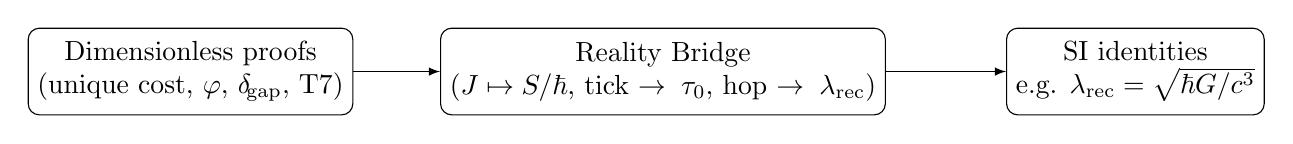
\begin{tikzpicture}[node distance=6cm,>=latex]
  \tikzstyle{block}=[draw,rounded corners,minimum height=1.1cm,minimum width=3.2cm,align=center]
  \node[block] (proofs) {Dimensionless proofs\\(unique cost, $\varphi$, $\delta_{\!\text{gap}}$, T7)};
  \node[block,right of=proofs] (bridge) {Reality Bridge\\($J\mapsto S/\hbar$, tick $\to\;\tau_0$, hop $\to\;\lambda_{\mathrm{rec}}$)};
  \node[block,right of=bridge] (si) {SI identities\\e.g. $\lambda_{\mathrm{rec}}=\sqrt{\hbar G/c^{3}}$};
  \draw[->] (proofs) -- (bridge);
  \draw[->] (bridge) -- (si);
\end{tikzpicture}
\caption{Pipeline: dimensionless proofs $\to$ single bridge $\to$ meter‑native (SI) identities.}
\label{fig:pipeline}
\end{figure}
\begin{table}[h]
\centering
\caption{Constants and SI hooks}
\label{tab:constants}
\begin{tabular}{@{}P{2.4cm} P{6.5cm} P{6.8cm}@{}}
\toprule
\textbf{Constant} & \textbf{Lean hook(s)} & \textbf{Semantics} \\
\midrule
\ph & \LeanHook{Constants.phi\_fixed\_point}; \LeanHook{Constants.phi\_sq\_eq\_phi\_add\_one} & Golden‑ratio fixed point and algebraic identity. \\
Gap $\delta$ & \LeanHook{Constants.delta\_gap}; \LeanHook{Constants.delta\_gap\_pos} & $\delta_{\!\text{gap}}=\ln\ph>0$. \\
Tick & \LeanHook{Constants.tau\_rec}; \LeanHook{Constants.tau\_rec\_eq\_pi\_over\_4\_logphi} & $\tau_{\mathrm{rec}}=(2\pi)/(8\ln\ph)$ (factor on $\tauzero$). \\
Speed $c$ & \LeanHook{Constants.c\_def}; \LeanHook{Constants.c\_pos} & $c=\ell_0/\tauzero$, positivity. \\
$\lamrec$ & \LeanHook{Constants.RSUnits.lambda\_rec}; \LeanHook{Constants.lambda\_rec\_sq} & $\lamrec=\sqrt{\hbar G/c^{3}}$; square form. \\
$\lamrec(\pi)$ & \LeanHook{Constants.RSUnits.lambda\_rec\_pi}; \LeanHook{Constants.lambda\_rec\_pi\_eq\_lambda\_rec\_div\_sqrt\_pi} & $\pi$‑normalized variant and linking lemma. \\
SI hooks & \LeanHook{Constants.RSUnits.lambda\_rec\_SI\_pi\_def}; \LeanHook{Constants.RSUnits.lambda\_rec\_SI\_pi\_rewrite\_c} & Calibration equalities for common anchor choices. \\
\bottomrule
\end{tabular}
\end{table}

\begin{table}[h]
\centering
\caption{Classical correspondences}
\label{tab:bridges}
\begin{tabular}{@{}P{4.1cm} P{6.4cm} P{5.0cm}@{}}
\toprule
\textbf{RS statement} & \textbf{Classical statement} & \textbf{Lean hook(s)} \\
\midrule
Discrete conservation & Continuity equation $\partial_t\rho+\nabla\!\cdot J=0$ (under coarse‑graining assumptions) & \LeanHook{ClassicalBridge.discrete\_to\_continuum\_continuity}; \LeanHook{ClassicalBridge.RiemannSum} \\
Gauge uniqueness (T4) & Potentials unique up to a constant on components & \LeanHook{ClassicalBridge.gaugeClass\_eq\_of\_same\_delta\_basepoint} \\
Variational (T5) & EL/log‑axis equivalence; convex minimum at $t=0$ & \LeanHook{Cost.T5\_EL\_equiv\_general} \\
\bottomrule
\end{tabular}
\end{table}

\begin{table}[h]
\centering
\caption{Spectra ratio identities}
\label{tab:spectra}
\begin{tabular}{@{}l P{7cm} P{5cm}@{}}
\toprule
\textbf{Name} & \textbf{Statement (sketch)} & \textbf{Lean hook(s)} \\
\midrule
Unified ratio (zpow) & $\displaystyle \frac{m(k_2,r_2)}{m(k_1,r_1)}=2^{\,k_2-k_1}\,\varphi^{\,r_2-r_1}$ & \LeanHook{Spectra.mass\_ratio\_zpow}; \LeanHook{Spectra.phi\_zpow} \\
$k$‑shift & One $k$‑step multiplies mass by $2$ & \LeanHook{Spectra.mass\_kshift} \\
$r$‑shift & One $r$‑step multiplies mass by $\varphi$ & \LeanHook{Spectra.mass\_rshift} \\
\bottomrule
\end{tabular}
\end{table}

\appendix
\section{Lemma/Definition Inventory}\label{app:lemmas}
Flat list of Lean anchors cited in the paper (one‑line descriptions).
\begin{itemize}[leftmargin=1.25em]
  \item \LeanHook{Cost.Jlog} — log‑axis form $J(\mathrm{e}^{t})=\cosh t - 1$.
  \item \LeanHook{Cost.hasDerivAt\_Jlog} — derivative facts on the log axis.
  \item \LeanHook{Cost.Jlog\_nonneg} — nonnegativity/convexity on the log axis.
  \item \LeanHook{Cost.T5\_EL\_equiv\_general} — EL equivalence for $F\circ\exp$ vs. $\cosh t-1$.
  \item \LeanHook{Cost.deriv\_Jlog\_zero}, \LeanHook{Cost.Jlog\_zero} — stationarity/minimum at $t=0$.
  \item \LeanHook{Constants.phi\_sq\_eq\_phi\_add\_one} — $\varphi^{2}=\varphi+1$.
  \item \LeanHook{Constants.phi\_fixed\_point} — $\varphi$ solves $x=1+1/x$.
  \item \LeanHook{Constants.fixed\_point\_unique\_pos} — uniqueness of the positive fixed point.
  \item \LeanHook{Constants.phi\_pos}, \LeanHook{Constants.one\_lt\_phi} — positivity, $\varphi>1$.
  \item \LeanHook{Constants.exp\_log\_phi} — $\exp(\ln\varphi)=\varphi$.
  \item \LeanHook{Constants.delta\_gap}, \LeanHook{Constants.delta\_gap\_pos} — ledger gap $\ln\varphi>0$.
  \item \LeanHook{Constants.tau\_rec}, \LeanHook{Constants.tau\_rec\_eq\_pi\_over\_4\_logphi}, \LeanHook{Constants.tau\_rec\_pos} — recognition tick.
  \item \LeanHook{Constants.c\_def}, \LeanHook{Constants.c\_pos} — $c=\ell_0/\tau_0$, positivity.
  \item \LeanHook{Constants.hbar\_def}, \LeanHook{Constants.hbar\_pos} — $\hbar$ definition/positivity (if present).
  \item \LeanHook{Constants.RSUnits.lambda\_rec}, \LeanHook{Constants.lambda\_rec\_def}, \LeanHook{Constants.lambda\_rec\_sq} — recognition length and square form.
  \item \LeanHook{Constants.RSUnits.lambda\_rec\_pi}, \LeanHook{Constants.lambda\_rec\_pi\_eq\_lambda\_rec\_div\_sqrt\_pi} — $\pi$‑normalized variant and link.
  \item \LeanHook{Constants.RSUnits.c\_SI}, \LeanHook{Constants.RSUnits.lambda\_rec\_SI\_pi\_def}, \LeanHook{Constants.RSUnits.lambda\_rec\_SI\_pi\_rewrite\_c}, \LeanHook{Constants.RSUnits.lambda\_rec\_SI\_pi\_SIbase}, \LeanHook{Constants.RSUnits.lambda\_rec\_SI\_pi\_with\_c\_of\_cal} — SI calibration lemmas.
  \item \LeanHook{Constants.Ecoh\_phi5}, \LeanHook{Constants.EcohDerived\_of\_Ecoh\_phi5} — symbolic $E_{\mathrm{coh}}=E_0\,\varphi^{-5}$ relation.
  \item \LeanHook{ClassicalBridge.CoarseGrain}, \LeanHook{ClassicalBridge.RiemannSum}, \LeanHook{ClassicalBridge.ContinuityEquation}, \LeanHook{ClassicalBridge.discrete\_to\_continuum\_continuity} — continuity bridge schema.
  \item \LeanHook{ClassicalBridge.gaugeClass\_eq\_of\_same\_delta\_basepoint} — gauge uniqueness up to a constant.
  \item \LeanHook{Spectra.B\_of}, \LeanHook{Spectra.mass}, \LeanHook{Spectra.B\_of\_pos}, \LeanHook{Spectra.mass\_pos} — mass law, positivity.
  \item \LeanHook{Spectra.mass\_strict\_mono\_k}, \LeanHook{Spectra.mass\_strict\_mono\_r} — monotonicity.
  \item \LeanHook{Spectra.phi\_zpow}, \LeanHook{Spectra.mass\_ratio\_zpow}, \LeanHook{Spectra.mass\_kshift}, \LeanHook{Spectra.mass\_rshift} — zpow‑unified ratios, shifts.
  \item \LeanHook{Spectra.mass\_using\_EcohDerived} — rewrite with the symbolic $E_{\mathrm{coh}}$ relation.
  \item \LeanHook{Constants.Sector}, \LeanHook{Constants.B\_of\_sector}, \LeanHook{Constants.B\_e}, \LeanHook{Constants.B\_q}, \LeanHook{Constants.B\_W} — sector factors and simplifications.
\end{itemize}

\section{Normalization Note (\texorpdfstring{$\lambda_{\mathrm{rec}}$}{lambda} vs. $\lambda_{\mathrm{rec}}(\pi)$)}\label{app:norm}
We document two common conventions and their equality via a Lean lemma.
\begin{itemize}[leftmargin=1.25em]
  \item Standard Planck‑form identity (bridge semantics):
  \[
    \lambda_{\mathrm{rec}}\;=\;\sqrt{\frac{\hbar\,G}{c^{3}}}\,.
  \]
  \item $\pi$‑normalized variant (documented convention):
  \[
    \lambda_{\mathrm{rec}}(\pi)\;=\;\frac{\lambda_{\mathrm{rec}}}{\sqrt{\pi}}\,.
  \]
  \item Linking lemma (Lean): \LeanHook{Constants.lambda\_rec\_pi\_eq\_lambda\_rec\_div\_sqrt\_pi}.
\end{itemize}
Calibration variants used in Section~\ref{tab:constants}:
\begin{itemize}[leftmargin=1.25em]
  \item Base SI (\,$\ell_{0}=1\,\mathrm{m},\,\tau_{0}=1\,\mathrm{s}$\,) — see \LeanHook{Constants.RSUnits.lambda\_rec\_SI\_pi\_SIbase}.
  \item Kinematic calibration (\,$\ell_{0}=c\_{\!\mathrm{SI}}\,\tau_{0}$\,) — see \LeanHook{Constants.RSUnits.lambda\_rec\_SI\_pi\_rewrite\_c} and \LeanHook{Constants.RSUnits.lambda\_rec\_SI\_pi\_with\_c\_of\_cal}.
\end{itemize}

\section{Artifact Guide (condensed)}\label{app:artifact}
\paragraph{Where.} Public repository: \href{\LeanRepoURL}{\LeanRepoURL}.\newline
\textbf{Pinned metadata:} tag \texttt{v0.1.0}; Lean \texttt{4.x}; Mathlib commit \texttt{<hash>}.

\paragraph{How to build.}
\begin{itemize}[leftmargin=1.25em]
  \item Install Lean~4 and Mathlib (standard instructions).
  \item Open \texttt{IndisputableMonolith.lean} in a Lean‑aware editor for on‑demand elaboration, or run \texttt{lake build} if a Lake package is present.
\end{itemize}

\paragraph{How to navigate.} Search for the lemma names listed in Appendix~\ref{app:lemmas}; names are frozen in the artifact. Example grep (ripgrep):
\begin{verbatim}
rg -n "phi_fixed_point|delta_gap|tau_rec|lambda_rec\
(|gaugeClass_eq|mass_ratio_zpow" IndisputableMonolith.lean
\end{verbatim}

\paragraph{CI/Audit (optional).} A simple script can check that every hook cited in the paper appears in the artifact and report success/failure. This is not required by the paper but simplifies artifact evaluation.

\begin{thebibliography}{99}
\bibitem{DeMouraUllrichLean4} Leonardo de Moura and Sebastian Ullrich. The Lean 4 Theorem Prover (system description). 2021.
\bibitem{mathlib2020} Jeremy Avigad et al. The Lean Mathematical Library. 2020.
\bibitem{Nipkow2002Isabelle} Tobias Nipkow, Lawrence C. Paulson, and Markus Wenzel. Isabelle/HOL: A Proof Assistant for Higher‑Order Logic. Springer, 2002.
\bibitem{Harrison2009HOLLight} John Harrison. HOL Light: An Overview. In Theorem Proving in Higher Order Logics, 2009.
\bibitem{CoqManual2023} The Coq Development Team. The Coq Proof Assistant Reference Manual. 2023.
\bibitem{Hales2017Flyspeck} Thomas Hales et al. A formal proof of the Kepler conjecture. Forum of Mathematics, Pi, 2017.
\bibitem{Leroy2009CompCert} Xavier Leroy. Formal verification of a realistic compiler. Communications of the ACM, 2009.
\bibitem{BoldoMelquiond2011Flocq} Sylvie Boldo and Guillaume Melquiond. Flocq: A unified library for proving floating‑point algorithms in Coq. In IEEE Transactions on Computers, 2011.
\bibitem{ACMArtifacts2020} ACM. Artifact Evaluation and Badging Version 1.1. 2020.
\bibitem{Harrison2013Euclidean} John Harrison. The HOL Light Theory of Euclidean Space. Journal of Automated Reasoning, 2013.
\end{thebibliography}

\end{document}
